\documentclass{article}
\usepackage[utf8]{inputenc}
\usepackage{geometry}
\usepackage{longtable}
\usepackage{graphicx} % For including images
\usepackage{hyperref} % For hyperlinks

\geometry{
 a4paper,
 total={170mm,257mm},
 left=20mm,
 top=20mm,
}

\title{Software Architecture of Train Inter Payment System (TrIP)}
\author{Group 04}
\date{\today}

\begin{document}

\maketitle
\newpage

\section*{Product Introduction}
The Train Inter Payment System (TrIP) is a collaborative project initiated by three railroad tycoons to streamline the payment process for train travel. These tycoons, operating a network connecting towns, industries, and a university, aim to address the interoperability issues of their existing payment systems. TrIP will feature smart payment terminals at each station, enabling direct communication for subscription validation or single-fare payments. This system, underpinned by a service-based architecture, involves critical components like payment terminals and tycoon-specific systems. It's designed with key stakeholder requirements in mind: maintainability and operational efficiency for the owner, usability and reliability for the tycoons, and usability and security for passengers. The project seeks to ensure passengers can easily manage payments and subscriptions across the network, enhancing the overall travel experience while safeguarding user data.

\newpage
\subsection{Decision 3: Routes management}

\subsection*{Status}
Accepted.

\subsection*{Architectural Summary}
% TODO

\subsection*{Concern}
The concern is to facilitate a seamless travel planning experience for passengers by ensuring the system can accurately and efficiently gather available route options from various tycoon systems and present them based on the user's criteria of price, time, and subscription status.

\subsection*{Context}
In the context of enhancing the TrIP system's ability to provide optimized travel options, we face the challenge of efficiently querying multiple tycoon systems to gather route information that aligns with passenger preferences and existing subscriptions.
The decision is centered on the system's interface with tycoon systems to retrieve and optimize route data, which impacts the functionality and performance of the terminal's route planning features for the passengers.

\subsection*{Criteria}
The key criteria for the decision include:
\begin{itemize}
    \item User-friendly passenger interface.
    \item Comprehensive and diverse route options.
    \item Accurate representation of options based on multiple factors.
    \item Streamlined integration with multiple tycoon systems.
\end{itemize}

\subsection*{Option 1: Direct Tycoon Integration}
Terminals directly interface with each tycoon system and the central database to collate route options. The route optimizer processes this data to present optimal travel solutions. This requires our system to have APIs to query each of the tycoons systems.
\begin{figure}[ht]
    \centering
    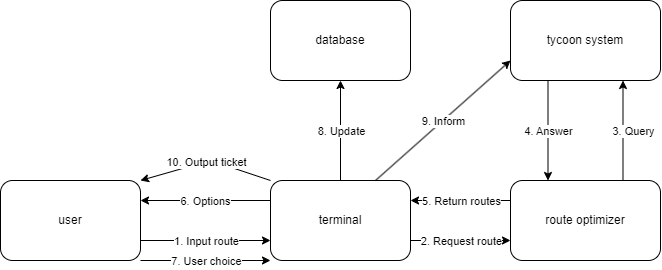
\includegraphics[width=\textwidth]{drawings/decision3_drawings/direct.png}
    \caption{Direct Data Management Interface}
    \label{fig:direct-data-interface}
\end{figure}

\subsection*{Option 2: Centralized Route Management Module}
A central route data management module acts as an intermediary between terminals and tycoon systems, standardizing and aggregating data before it is processed by the route optimizer. A database containing the timetables will be kept up to date by the tycoon (possibly though an API, this will be the focus of a later decision). The route data management system might cache optimized routes, in order to minimize database requests. A module specialized in running optimizations with the data it is provided with interacts solely with the Route Management Module.
\begin{figure}[ht]
    \centering
    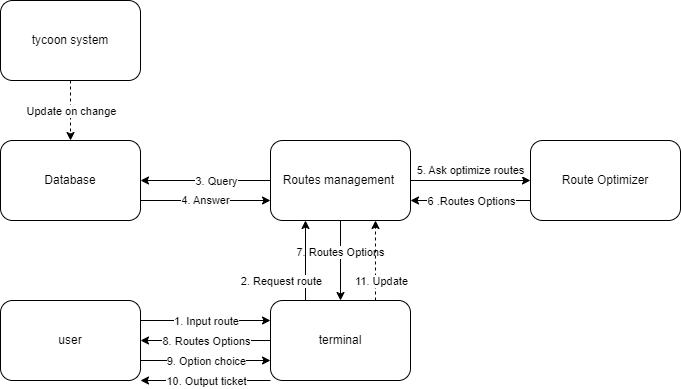
\includegraphics[width=\textwidth]{drawings/decision3_drawings/centralized.png}
    \caption{Centralized Route Management Module. Dashed lines represents steps to be explained in future decisions.}
    \label{fig:centralized-data-interface}
\end{figure}
  
\subsection*{Decision}
We have decided to proceed with Option 2: Centralized Route Management Module. This decision is based on the module's ability to simplify the data flow between systems and to effectively manage the complexity of integrating with multiple tycoon systems. The introduction of a separate data management module will allow for greater flexibility and scalability.

\subsection*{Consequences}
\textbf{Positive Consequences:}
\begin{itemize}
    \item Simplified data flow between the trip system and tycoons.
    \item Improved scalability and maintainability of the system.
    \item Easier to integrate with current and future tycoon systems.
\end{itemize}
\textbf{Negative Consequences:}
\begin{itemize}
    \item Initial development and integration effort for the new module.
    \item Potential complexity in data synchronization between modules.
\end{itemize}
This approach is expected to provide a solid foundation for the system's scalability and adaptability to evolving requirements and stakeholder needs.
\newpage

\subsection{Decision 4: Account and Subscriptions management}

\subsection*{Status}
Accepted.

\subsection*{Architectural Summary}


\subsection*{Concern}
A user wants to traver around the network using its subscription(s) instead of always having to buy a single fare.
Tycoons have explicitely requested to maintain their own subscriptions separated.
The following user stories are tied to this decision:
\begin{itemize}
    \item \textbf{User Story 16}: 16. As a passenger, I want to be able to purchase a single ticket that allows me to travel across all train networks so that I can travel seamlessly without needing to buy separate tickets for each tycoon's network.
    \item \textbf{User Story 23}: As a tycoon, I want the payment system to integrate with my existing infrastructure with minimal disruption so that I can maintain high service levels during the transition..
\end{itemize}

Specific concerns identified for the system include the following:
\begin{itemize}
    \item A passenger should be able to have different subscriptions for the three tycoons.
    \item Each of the three tycoon wants to have its own subscription fee system.
\end{itemize}

\subsection*{Context}
In developing the TrIP system, we explore subscription model architectures that align railway tycoons' need for flexibility with passengers' demand for simplicity. 
We assess the trade-offs between unified and tycoon-specific models to enhance both operational autonomy and passenger convenience.
When passengers want to go from station A to station B, they want to be able to use all the subscription they have and pay for the trains belonging to tycoons they are not subsribed to.
The terminal has to communicate with the tycoon systems to verify subscriptions and check routes.
Alternatively, if passengers have active subscriptions to a tycoon, they should be allowed onboard the train without a ticket. 

\subsection*{Criteria}
\begin{itemize}
\item Ease of use for the passenger.
\item Multiple route options for the user.
\item The system returns to user usable options based on price/time/availability/subscription.
\item Simple integration with the tycoon systems.
\end{itemize}

\subsection*{Option 1: Introduction of a subscription manager tool, route management needs to take subs into consideration.}
We want to include a Subscription Manager module to our functional view. 
Such a module has the responsibility to verify subscriptions, communicating with the tycoon system.
It should also allow users to create their own TRIP account and tie it to subscriptions.
Since we need scalability, we consider using a TRIP account that is tied to one or many subscriptions, and let the user add new or automatically renew the existing ones.
This means that we need an authentication means, like a magnetic card, or a phone app linked to NFC scanning or other alternatives.
This will be the topic of a future decision.
Furthermore, the Route management module needs to be able to optimize with respect to price, given that the passenger holds some subscription.
The idea is to add an optional initial iteration to the sequence of actions sketched in decision 3.
This requires a way to communicate the subscription to the terminal, be it a QR code, a code or a magnetic card. 
This should be the topic of another decision.

\subsection*{Pros}

\begin{itemize}[noitemsep]
    \item \textbf{Modular Architecture:} The separation of subscription management and route optimization into distinct modules enhances the system's modularity, making it easier to maintain, update, or replace parts of the system without affecting others.
    \item \textbf{Scalability:} Designed with scalability in mind, allowing for easy addition and management of new subscriptions or renewal of existing ones, which can accommodate growing user demands and evolving business requirements.
    \item \textbf{Reduced Risk of System-wide Failures:} By distributing functionalities across different systems or modules, the impact of a failure in one component is limited, reducing the risk of system-wide outages and improving overall system reliability.
    \item \textbf{Flexibility in User Authentication:} Supports various means of user authentication (e.g., magnetic card, smartphone app), offering flexibility and convenience for users to access their subscriptions and travel seamlessly.
\end{itemize}

\subsection*{Cons}

\begin{itemize}[noitemsep]
    \item \textbf{Increased System Interactions:} The decoupled nature of the system requires more interactions between separate modules (e.g., subscription verification and route optimization), which can increase the complexity of integration and potentially lead to higher latency in response times.
    \item \textbf{Integration Complexity:} Ensuring seamless communication and data consistency between different modules can introduce additional complexity in system integration and require more sophisticated coordination mechanisms.
    \item \textbf{Higher Overhead:} Managing separate systems for subscription and route optimization may lead to higher operational overhead in terms of both system resources and administrative efforts to maintain multiple components.
\end{itemize}
% The functional view schema is in my bag. TODO

\subsection*{Option 2: Integrated Subscription-Route Optimization Service}
The Integrated Subscription-Route Optimization Service (IS-ROS) combines the functionality of subscription management and route optimization into a single service. 
\subsubsection*{Pros}
\begin{itemize}[noitemsep]
    \item \textbf{Performance} Streamlines the process by combining two functionalities, potentially reducing response time for route optimization.
    \item \textbf{Reduced Interactions between systems} Simplifies the architecture by reducing the number of interactions between separate systems.
\end{itemize}
\subsubsection*{Cons}
\begin{itemize}[noitemsep]
    \item \textbf{Increased Complexity within Single Module} Increases complexity within a single system, which may require more resources to develop and maintain.
    \item \textbf{Failures have larger impact} May lead to higher dependency on a single system, which can be a point of failure if the system goes down.
\end{itemize}

\subsection*{Decision}
We decided to pick Option 1. The increased concern for scalability, caused by event 1, points clearly to the listed pros of this option. Furthermore, the focus on modularity
gives us easy maintenability, which is important for the TRIP owner.
Performance in this case doesn't seem to be that central, as optimization of routes should be precomputed and cached, given that timetables should not change often and that subscription have relatively long lasting periods.
With our option, we still have the flexibility to assign more computational or data access resources to the module who needs them the most.

\subsection*{Consequences}
\subsection*{Positive Consequences}

\begin{itemize}[noitemsep]
    \item \textbf{Enhanced Scalability:} Modular design facilitates easy scaling and integration of new features.
    \item \textbf{Improved Maintainability:} Simplifies updates and troubleshooting, allowing for technology-specific optimizations within each module.
    \item \textbf{Reduced System-wide Failure Risk:} Isolates failures to individual modules, enhancing overall system reliability.
\end{itemize}

\subsection*{Negative Consequences}

\begin{itemize}[noitemsep]
    \item \textbf{Increased System Complexity:} Necessitates sophisticated coordination and integration, potentially introducing latency.
    \item \textbf{Higher Initial Costs:} Development and maintenance of separate modules may lead to higher initial and operational costs.
    \item \textbf{Data Consistency Challenges:} Requires robust synchronization mechanisms to ensure data consistency across modules.
\end{itemize}


\newpage

\subsection{Decision 5: How to Handle Quickly Filling Trains?}

\subsection*{Status}
Accepted

\subsection*{Architectural Summary}
\textit{[Provide a brief summary of the architectural context and the specific system components affected by this decision.]}

\subsection*{Concern}
Ensuring a high level of usability and availability in the ticketing system is paramount. System operators and railroad tycoons aim to minimize customer service issues arising from passengers' frustrations with paying for unavailable routes.
\begin{itemize}
    \item \textbf{User Story 15}: Concerns about paying for unavailable routes.
    \item \textbf{User Story 26}: The need for real-time updates on train schedules.
    \item \textbf{User Story 27}: Integration with maintenance scheduling for minimal service disruption.
\end{itemize}

\subsection*{Context}
This decision seeks to address challenges associated with quickly filling trains, especially during peak hours, to offer a seamless and fair ticket purchasing experience. Mitigating the risk of overbooking and enhancing passenger satisfaction are central goals. It's critical to efficiently manage simultaneous requests for the last available seats to ensure a positive experience for commuters and students who rely on timely and available transportation.

\subsubsection*{QA scenario}
The following outlines a Quality Attribute (QA) scenario focusing on the real-time seat availability and booking process during peak hours. This scenario is structured to evaluate the system's usability and performance under conditions of high demand.
\paragraph{Source} Passenger interacting with a payment terminal (or any other way of booking tickets, e.g. an app or a website).
\paragraph{Stimulus} Two passengers try to buy the same ticket.
\paragraph{Artifact} The \textit{data management system}, \textit{database maintaining seat availability information} and the \textit{user interface} the passenger interacts with.
\paragraph{Response} Upon receiving the stimulus, the system's response is to immediately check the current availability of the selected seat, lock the seat for the passenger if it is available (thus preventing other bookings), and provide real-time feedback to the passenger regarding the seat's status (e.g., locked for purchase, already taken). If the seat is available and locked for the passenger, the system then proceeds with the payment process.
\paragraph{Response Measure}[\textit{After the decision is taken}] The effectiveness of the system's response is measured as follows:
\begin{itemize}
    \item Percentage of purchases ending with passengers buying the same ticket. This can be measured by a customer service.
\end{itemize}

\subsection*{Criteria}
\begin{itemize}
    \item Minimize excessive requests to tycoon systems, avoiding system overload.
    \item Ensure high performance to prevent a negative user experience.
    \item Prevent multiple users from paying for the same seat, ensuring fairness in ticket sales.
\end{itemize}

\subsection*{Option 1: Lock the Seats Before Payment}
We should maintain a database where info about scheduled trains is stored. This database should be updated by the terminal when a ticket has been bought. The database should ask periodically for updates on schedules from the tycoon systems. When a user selects that they want to pay for a specific ticket, that ticket should be locked, so that no one else can buy it. If the payment is not ultimated, it can be unlocked. Note that it can still happen that due to maintenance, a train is cancelled last minute. 

% TODO: What happens with the customer service? Should we add it to the context view? They will for sure need info from us, like who paid and how much. These should be two future decisions (how to deal with customer service in case of train disruptions, how to keep up to date about disruptions).

\subsubsection*{Pros}
\begin{itemize}[noitemsep]
    \item \textbf{Fairness} (Usability, Availability): Ensures that once a customer selects a ticket, it is reserved for them, preventing others from buying it.
    \item \textbf{Reduced System Load} (Performance, Efficiency): By locking seats before payment, it reduces the chances of multiple users attempting to pay for the same seat, thereby reducing system load.
\end{itemize}
\subsubsection*{Cons}
\begin{itemize}[noitemsep]
    \item \textbf{Potential for Seat Hoarding} (Usability, Efficiency): Customers might lock seats without completing the purchase, leading to temporarily reduced availability.
    \item \textbf{Increased Complexity} (Maintainability, Scalability): Managing locked seats, especially determining when to release them if payment is not completed, adds complexity.
\end{itemize}
\subsubsection*{User stories}
\begin{itemize}
    \item Directly addresses \textbf{User Story 15} by preventing payments for unavailable seats.
    \item Indirectly supports \textbf{User Stories 26 and 27} by contributing to system usability and reducing overbooking, though it does not directly offer real-time updates or integration with maintenance scheduling.
\end{itemize}

\subsection*{Option 2: Lock the Seats After Payment, FCFS, Refuse Payments if Seat is Booked}
Seats are locked only after payment confirmation, adhering to a first-come, first-served (FCFS) approach. This method ensures that seats are sold to passengers who complete the payment process first, minimizing the potential for holding seats unnecessarily.

\subsubsection*{Pros}
\begin{itemize}[noitemsep]
    \item \textbf{Efficiency} (Performance): Minimizes the time seats are unnecessarily held, as they are only locked upon payment completion.
    \item \textbf{Simplicity} (Maintainability): Easier to implement and maintain than preemptive locking mechanisms.
\end{itemize}
\subsubsection*{Cons}
\begin{itemize}[noitemsep]
    \item \textbf{User Experience} (Usability): Customers may go through the payment process only to find out the seat has been taken, leading to frustration.
    \item \textbf{Race Conditions} (Reliability): Higher risk of race conditions where multiple users complete payments for the last seat simultaneously.
\end{itemize}

\subsubsection*{User stories}
\begin{itemize}
    \item Aims to ensure fairness in seat allocation (\textbf{User Story 15}) by adhering to a first-come, first-served basis, reducing the risk of paying for unavailable seats.
    \item Does not directly address \textbf{User Stories 26 and 27}, but supports system performance and minimizes unnecessary seat holds.
\end{itemize}

\subsection*{Option 3: Real-time Seat Availability with Dynamic Allocation}
This option introduces a system for real-time tracking and dynamic allocation of seats. It involves continuous synchronization with tycoon systems to update seat availability instantly. The system could allow for a slight overbooking based on historical no-show rates, with safeguards in place to manage overbooked scenarios, such as offering alternative transportation options or compensation.

\subsubsection*{Pros}
\begin{itemize}[noitemsep]
    \item \textbf{Real-time Updates} (Availability, Usability): Enhances user experience by providing immediate feedback on seat availability.
    \item \textbf{Adaptability} (Scalability, Reliability): Can dynamically adjust to changing conditions, like cancellations or no-shows.
\end{itemize}
\subsubsection*{Cons}
\begin{itemize}[noitemsep]
    \item \textbf{Complex System Integration} (Maintainability, Operability): Requires continuous synchronization with external systems, increasing complexity.
    \item \textbf{Potential for Overbooking} (Usability, Reliability): While overbooking can be managed, it may lead to negative customer experiences.
\end{itemize}
\subsubsection*{User stories}
\begin{itemize}
    \item Directly solves \textbf{User Story 15}'s issue by ensuring passengers only pay for available seats and addresses \textbf{User Story 26} by providing real-time updates on train schedules.
    \item Supports \textbf{User Story 27} through dynamic allocation that can adjust to maintenance schedules, minimizing service disruptions.
\end{itemize}

\subsection*{Option 4: 2PC Protocol}
The Two-Phase Commit (2PC) protocol is a distributed transaction protocol that ensures all parts of a transaction across multiple systems either complete successfully or fail altogether. It is particularly useful in environments requiring strong consistency and atomicity, such as train terminal payment systems handling ticket purchases.

\subsubsection*{Pros}
\begin{itemize}[noitemsep]
    \item \textbf{Atomicity and Consistency} (Reliability, Consistency): 2PC guarantees that a transaction across distributed components either fully commits or fully aborts, maintaining the integrity and consistency of the database.
    \item \textbf{Fault Tolerance} (Availability, Reliability): By ensuring that all components agree on a transaction's outcome, 2PC enhances the system's ability to recover from partial failures without losing data integrity.
    \item \textbf{Coordination} (Integrity, Consistency): 2PC effectively coordinates complex transactions across multiple systems, ensuring that all parts of the transaction are synchronized.
\end{itemize}

\subsubsection*{Cons}
\begin{itemize}[noitemsep]
    \item \textbf{Performance Overhead} (Performance, Efficiency): The two-phase nature of the protocol can introduce latency, as it requires all participants to lock resources and wait for global commit or abort decisions.
    \item \textbf{Resource Locking} (Availability, Scalability): 2PC requires resources to be locked during the transaction, which can decrease system availability and limit scalability due to locking contention.
    \item \textbf{Complexity} (Maintainability, Operability): Implementing and maintaining a 2PC system introduces complexity, requiring robust failure and recovery mechanisms, and can complicate system operations and maintenance.
    \item \textbf{Risk of Blocking} (Availability): In cases where the coordinator fails after initiating the transaction but before completing it, participants can be left in a blocking state, waiting indefinitely for a decision and thus affecting system availability.
\end{itemize}
\subsubsection*{User stories}
\begin{itemize}
    \item Indirectly supports \textbf{User Story 15} by ensuring transactional integrity, which is foundational for reliable seat booking but does not directly address usability concerns.
    \item Does not directly address \textbf{User Stories 26 and 27}, but by ensuring consistent and reliable transactions, it lays the groundwork for future enhancements that could.
\end{itemize}

\subsection*{Decision}
In light of the trade-off analysis performed for each Option listed above, we decided to take Option 1. 
This Option ensures a solution to \textbf{User Story 15}, by effectively preventing two users to buy the same tickets. 
It is also good for reliability, a focus of the tycoons and for the usability required by the passengers, as they don't have to restart the booking procedure in case of failed payment.
Other options can lead to overbooking, which is unwanted given the concerns of passengers and tycoons.
Option 4 can be useful if the system is decentralized, but introduces unwanted complexity.

\subsection*{Consequences}
\textbf{Positive Consequences:}
\begin{itemize}
    \item Improved passenger experience through fair and efficient seat allocation.
    \item Reduced customer service issues related to overbooking and ticket availability.
    \item Enhanced system resilience against peak demand scenarios.
\end{itemize}
\textbf{Negative Consequences:}
\begin{itemize}
    \item Potential increase in system complexity and operational costs.
    \item Challenges in accurately forecasting demand for dynamic seat allocation or overbooking strategies.
    \item Possible passenger dissatisfaction in cases of overbooking or changes in train schedules.
\end{itemize}
\newpage

\subsection{Decision 6: Database scope and organization}

\subsection*{Status}
Review.

\subsection*{Architectural Summary}


\subsection*{Context}
We need to answer the following questions:
\begin{itemize}
\item Which info do we keep in the database? 
\item Do we need one or many databases?
\item How do we handle data protection?
\item How do we handle data update from tycoons/station management? (maybe for another decision?)
\end{itemize}

\subsection*{Concern}
We need to keep some information available from our system, but security of the data (especially payment and account data) is crucial for the government and for the passengers concerns.

\subsubsection*{User stories}
The following user stories are particularly relevant to the decision on the database scope, emphasizing the need for comprehensive management of subscriptions, security, and system integration:

\begin{itemize}[noitemsep]
    \item \textbf{User Story 1:} As a frequent traveler, I want to subscribe to a comprehensive monthly pass that includes all three networks so that I can save money on my regular commutes.
    
    \item \textbf{User Story 2:} As a passenger, I want to be able to check the balance of my multi-network travel card online so that I can easily manage my travel expenses.
    
    \item \textbf{User Story 3:} As a passenger with a subscription, I want to receive automatic notifications about my subscription renewal and any discounts or promotions available so that I can take advantage of cost savings. 
    
    \item \textbf{User Story 4:} As a tech-savvy passenger, I want to use a mobile app to manage my subscriptions, make payments, and receive digital tickets so that I can have a paperless and convenient travel experience. 
    
    \item \textbf{User Story 5:} As a passenger interested in sustainability, I want the system to track my travel carbon footprint and offer carbon offset options so that I can make environmentally responsible travel choices.
    
    \item \textbf{User Story 6:} As a passenger with mobility challenges, I want the payment system to provide information on accessible services and allow for easy purchase of accessible seating across all networks so that I can travel comfortably and safely.
    
    \item \textbf{User Story 16:} As a passenger, I want to be able to purchase a single ticket that allows me to travel across all train networks so that I can travel seamlessly without needing to buy separate tickets for each tycoon's network.
    
    \item \textbf{User Story 18:} As a government regulator, I want the payment system to adhere to data protection and financial transaction security standards so that passengers' personal and financial information is secure.
    
    \item \textbf{User Story 23:} As a tycoon, I want the payment system to integrate with my existing infrastructure with minimal disruption so that I can maintain high service levels during the transition.
    \item 
    \item \textbf{User Story 27:} As a network maintenance planner, I want the payment system to integrate with maintenance scheduling tools so that I can plan work with minimal disruption to the train service and revenue.
\end{itemize}

\subsection*{Option 1: Querying modules or external parties should know as little as possible}
We try to have one database for each important set of information that the system needs to know.
We try to stick to the Separation of Concerns principle, so that each module only has access to the data it scricly needs to operate.
We divide the following:
\begin{itemize}
    \item A database containing the timetable, the prices of seats and the bookings.
    \item A database containing the optimized routes cached after being calculated by the Routes Optimization Module.
    \item A database containing info about the accounts and their subscriptions. 
    \item A database recording payments that have been done, which should be accessed in case for example of complaints. 
\end{itemize}
\begin{figure}[ht]
    \centering
    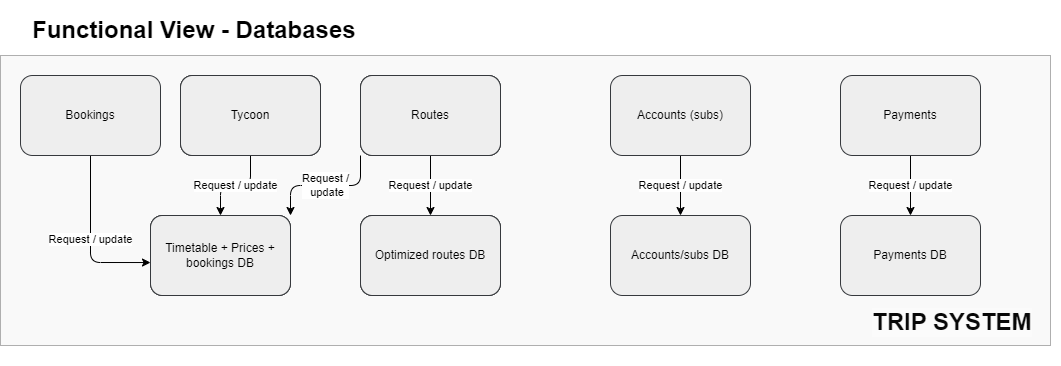
\includegraphics[width=\textwidth]{drawings/views_draft2/functional_view databases.png}
    \caption{Division of databases and their interaction with modules or stakeholders.}
    \label{fig:databases_view}
\end{figure}

\subsubsection*{Pros}
\begin{itemize}[noitemsep]
    \item \textbf{Enhanced Security} (Data Protection, Privacy): By segregating data across multiple databases, sensitive information is better protected, and access can be tightly controlled on a need-to-know basis.
    \item \textbf{Specialized Optimization} (Performance, Efficiency): Dedicated databases allow for optimization specific to their function, such as faster queries for timetable and booking data versus complex route optimization calculations.
\end{itemize}

\subsubsection*{Cons}
\begin{itemize}[noitemsep]
    \item \textbf{Increased Maintenance Overhead} (Maintainability, Complexity): Managing multiple databases adds complexity to the system's architecture, requiring more resources for maintenance and potentially higher costs.
    \item \textbf{Data Synchronization Challenges} (Reliability, Consistency): Ensuring data consistency across different databases can be challenging, especially in real-time, and may affect the system's overall reliability.
\end{itemize}

\subsection*{Option 2: Unified Centralized Database System}

This option proposes a centralized database architecture that consolidates all necessary information into a single, unified database system. It incorporates robust access control layers to manage data access based on module or user roles, ensuring that each part of the system accesses only the data it needs for operation. This model simplifies data management, enhances security through centralized control mechanisms, and facilitates easier updates and integrations. This model can be improved with having accounts database as a separate component, and keeping the rest of the databases central. In this way accounts data will be secure, and the rest of the systems will access accounts data anonymously via ids. Manage permissions for eacsh tycoon, on which info they can access (they shouldn't be able to connect name to bank account). In this way we can keep everything in the same place, but each tycoon api will have specificed access protocols. Tycoons can only update timetables and prices.

We can keep bookings data a DaaS, since it needs to be updated regularly and concurrently. Rest can be a server based database. Since we can cache routes we don't want cloud services for these. 

\subsubsection*{Pros}
\begin{itemize}[noitemsep]
    \item \textbf{Simplified Data Management} (Maintainability, Efficiency): Centralizing data storage simplifies the architecture by reducing the number of systems to manage, making it easier to maintain and update the database.
    \item \textbf{Improved Data Consistency} (Reliability, Integrity): A unified database ensures that all modules access the most current and consistent data, reducing the risk of discrepancies and errors.
    \item \textbf{Enhanced Integration Capability} (Scalability, Interoperability): With all data in one place, integrating new features, modules, or external systems becomes more straightforward, promoting scalability and interoperability.
\end{itemize}

\subsubsection*{Cons}
\begin{itemize}[noitemsep]
    \item \textbf{Risk of a Single Point of Failure} (Reliability, Availability): Centralizing data creates a single point of failure, which could potentially lead to system-wide outages affecting all functionalities if the database goes down.
    \item \textbf{Scalability Concerns} (Performance, Scalability): As the system grows, a centralized database might struggle with performance issues due to the increasing volume of data and concurrent access requests.
    \item \textbf{Complexity in Ensuring Data Protection} (Security, Privacy): Protecting a large, centralized repository of sensitive information poses significant challenges, requiring robust security measures to prevent unauthorized access and data breaches.
\end{itemize}

\subsection*{Option 3: Database per tycoon or not}

\subsubsection*{Pros}
\begin{itemize}[noitemsep]
    \item \textbf{Tycoon specific features} 
    \item \textbf{Tycoon access permissions are automatically managed} 
\end{itemize}

\subsubsection*{Cons}
\begin{itemize}[noitemsep]
    \item \textbf{Hard to manage the database} 
    \item \textbf{Shared data is potentially doubled} 
\end{itemize}

\subsection*{Option 4: Hybrid cloud storage}
Crucial data stored in cloud (timetables, and prices and bookings). Non-crucial data (accounts, payments) gets stored in non-cloud database one per tycoon, such that they can only access their own customer data.

\subsubsection*{Pros}
\begin{itemize}[noitemsep]
    \item \textbf{Tycoon specific access for accounts data} 
    \item \textbf{Secure and qucik access to data crucial data} 
    \item \textbf{Cheap storage for non-crucial data} 
\end{itemize}

\subsubsection*{Cons}
\begin{itemize}[noitemsep]
    \item \textbf{Can get expensive} 
    \item \textbf{Implementation of two different database types and their interactions setup}
\end{itemize}

\subsection*{Decision}
We choose Hybrid cloud storage System, increased Availability which is important for event 2 which requirees less stringent Maintainability and cost requirements. Cloud increased cost and interaction between databases increase Maintainability compared to single database.
\subsection*{Consequences}
\textbf{Positive Consequences:}
\begin{itemize}
    \item \textbf{database as a service}: Single point of failure is reduced, scalable.
    \item \textbf{}: Single point of failure is reduced, scalable.
\end{itemize}
\textbf{Negative Consequences:}
\begin{itemize}
    \item \textbf{Tycoon permission management} : More complextiy, we need to restrict access for each tycoon.
    \item \textbf{Single point of failure} : If database fails, everything fails.(bad for availablity)[maybe a solution is backup database].
    \item \textbf{database as a service}: Expensive.
\end{itemize}
\newpage

\subsection{Decision 7: Customer Service}

\subsection*{Status}
Open

\subsection*{Architectural Summary}

\subsection*{Concern}
The primary concern is to ensure that customer service representatives have access to accurate and timely information to address passenger queries and resolve issues efficiently, without compromising data privacy.

\subsection*{Context}
This decision outlines the strategy for communication between the TrIP system and customer service teams to facilitate rapid and effective resolution of customer issues.
Customer service teams require real-time access to passenger data, ticketing information, and system status to provide informed support. The chosen communication strategy must balance the need for information accessibility with system security and data privacy regulations.

\subsection*{Criteria}
\begin{itemize}
    \item Timeliness and accuracy of information communicated.
    \item Data privacy and security compliance.
    \item Ease of access for customer service representatives.
    \item Minimization of system complexity and maintenance.
    \item Integration with existing customer service platforms.
    \item Cost-effectiveness of the communication solution.
\end{itemize}

\subsection*{Option 1: Direct Access to Live Data}
Grant customer service representatives direct access to the live operational database with appropriate read-only permissions and privacy safeguards in place.

\subsection*{Option 2: Periodic Data Sync to a Dedicated Customer Service Database}
Regularly synchronize relevant data from the operational database to a separate customer service database designed for query efficiency and tailored access control.

\subsection*{Option 3: On-Demand Data Retrieval via Secure API}
Implement a secure API that allows customer service representatives to retrieve necessary data on-demand while maintaining strict access controls and audit trails.

\subsection*{Option 4: Automated Reporting System}
Develop an automated reporting system that provides customer service representatives with pre-defined reports and dashboards, reducing the need for direct data access.

\subsection*{Decision}
Option 3 is chosen: not enough requests to justify the burden of an additional db. option4 requires to much work from us. Option 1 doesnt seem secure enough.

\subsection*{Consequences}
\textbf{Positive Consequences:}
\begin{itemize}
    \item Option 1: Immediate access to data allows for quick customer service responses.
    \item Option 2: Data syncing provides a stable environment tailored for customer service needs.
    \item Option 3: Secure API ensures data privacy and minimizes unnecessary data exposure.
    \item Option 4: Automated reports streamline the information delivery process.
\end{itemize}
\textbf{Negative Consequences:}
\begin{itemize}
    \item Option 1: Direct access to live data could pose security risks if not managed correctly.
    \item Option 2: Data syncing could lead to delays in information relay if not frequent enough.
    \item Option 3: On-demand retrieval may introduce latency and requires robust API management.
    \item Option 4: Automated reporting may not cover all ad-hoc queries from customer service representatives.
\end{itemize}
% TODO: move options pros and cons to the options subsections.
\newpage
\section*{Decision 8: Serverless vs. Servers for calculations}

\subsection*{Status}

\subsection*{Architectural Summary}


\subsection*{Concern}


\subsection*{Context}


\subsection*{Criteria}
\begin{itemize}
\end{itemize}

\subsection*{Option 1: Serverless}
You dont deal with servers.

\subsection*{Option 2: Servers}
Data is not shared with third party.

\subsection*{Decision}

\subsection*{Consequences}
\textbf{Positive Consequences:}
\begin{itemize}
\end{itemize}
\textbf{Negative Consequences:}
\begin{itemize}
\end{itemize}
\newpage



% \begin{table}[H]
    \resizebox{\textwidth}{!}{%
    \begin{tabular}{|l|c|c|c|c|c|c|c|c|c|c|c|}
    \hline
    \textbf{User Story} & \textbf{Usability} & \textbf{Performance} & \textbf{Security} & \textbf{Modifiability} & \textbf{Deployability} & \textbf{Energy Efficiency} & \textbf{Availability} & \textbf{Safety} & \textbf{Integrability} & \textbf{Testability} & \textbf{Accessibility} \\
    \hline
    1. Frequent traveler monthly pass & + &  &  &  &  &  &  &  &  &  &  \\
    \hline
    2. Check travel card balance & + &  &  &  &  &  &  &  &  &  &  \\
    \hline
    3. Subscription notifications & + &  &  &  &  &  &  &  &  &  &  \\
    \hline
    4. Mobile app management & + &  &  &  & - &  &  &  &  &  &  \\
    \hline
    5. Carbon footprint tracking &  & - &  &  &  & + &  &  &  &  &  \\
    \hline
    6. Accessible services info & + &  &  &  &  &  &  & + &  &  &  \\
    \hline
    7. Voice-activated features & + &  &  & - & - &  &  &  &  &  & + \\
    \hline
    8. Simple interface for elders & + &  &  & + &  &  &  &  &  &  &  \\
    \hline
    9. Multilanguage options & + &  &  & - &  &  &  &  &  &  &  \\
    \hline
    10. Quick access to popular trips & + & - &  & - &  &  &  &  &  &  &  \\
    \hline
    11. Scan student card for benefits & + &  &  & - &  &  &  &  &  &  &  \\
    \hline
    12. Single transaction for subscriptions & + & - &  &  &  &  &  &  &  &  &  \\
    \hline
    13. Charge train cards at terminal & + &  &  & - &  &  &  &  &  &  &  \\
    \hline
    14. Interface for visually impaired & + &  &  &  &  &  &  &  &  &  & + \\
    \hline
    15. Block payment for blocked routes & + & - &  & - &  &  &  &  &  &  &  \\
    \hline
    16. Single ticket across all networks & + & - &  & - &  &  &  &  &  &  &  \\
    \hline
    17. Subscriptions advice for commuting & + & - &  & - &  &  &  &  &  &  &  \\
    \hline
    18. Adherence to security standards &  &  & + & - &  &  &  &  & - & - &  \\
    \hline
    19. Detailed reporting for government & + &  &  & - &  &  &  &  & - &  &  \\
    \hline
    20. Reduced fares for eligible populations & + & - &  & - &  &  &  &  &  &  &  \\
    \hline
    21. Revenue tracking for tycoons & + & - &  & - &  &  &  &  &  &  &  \\
    \hline
    22. Exclusive promotions & + &  &  & - &  &  &  &  &  &  &  \\
    \hline
    23. Payment system integration & + &  &  & - &  &  &  &  & + & - &  \\
    \hline
    24. Access to analytics &  &  &  & - &  &  &  &  & + &  &  \\
    \hline
    25. Assistance for ticket purchases & + &  &  & - &  &  &  &  &  &  &  \\
    \hline
    26. Temporary fare adjustments &  &  &  & - &  & + &  &  &  &  &  \\
    \hline
    27. Integration with maintenance tools &  &  &  & - &  & + &  &  &  &  &  \\
    \hline
    28. Audit trails and compliance &  &  &  & - &  &  &  &  &  &  &  \\
    \hline
    \end{tabular}%
    }
    \caption{User Stories and Quality Attributes}
\end{table}

\section*{Context Viewpoint}
\subsection*{View: \textless{}Name\textgreater{}}
\subsubsection*{Model}
Place here the model representation of the view

\subsubsection*{Description}
Short description of the view

\subsubsection*{Glossary of Elements}
\begin{longtable}{lll}
Id & Name & Description \\
\end{longtable}

\subsection*{Analysis on Perspectives}
Describe how the view satisfies the different perspectives. 

\section*{Functional Viewpoint}

\section*{Information Viewpoint}

\section*{Concurrency Viewpoint}

\section*{Development Viewpoint}

\section*{Deployment Viewpoint}

\end{document}
